\documentclass[12pt, a4paper]{article}
\usepackage[utf8]{inputenc}
\usepackage{amsrefs}
\usepackage{tikz, wasysym}
\usetikzlibrary{automata,positioning}
\usepackage[]{algorithm2e}
\usepackage[]{csquotes}

\author{Sven Fiergolla}
\title{Wissenschaftliches Arbeiten mit \LaTeX}
\date{\today}

\begin{document}
 
\maketitle
%\pagebreak
\tableofcontents

%\chapter{Wissenschaftliche Arbeiten}
\paragraph{Abstract}
Dies ist eine Zusammenfassung über die Enstehung von wissenschftlichen Arbeiten als solches, sowie den dabei notwendigen Einsatz von \LaTeX \ zur Ausarbeitung.
\section{Einführung}

\section{Wissenschaftliche Arbeiten}


%\chapter{\LaTeX}
\section{Funktionalität von \LaTeX}
\subsection{Graphen}
\paragraph{}
1.Graph


	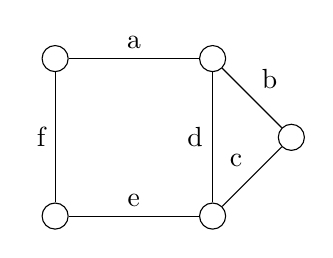
\begin{tikzpicture}[node distance=5cm,on grid,auto]
   
   \node[shape=circle,draw=black] (1) at (0,0) {};
   \node[shape=circle,draw=black] (2) at (0,2) {};
   \node[shape=circle,draw=black] (3) at (2,0) {};
   \node[shape=circle,draw=black] (4) at (2,2) {};
   \node[shape=circle,draw=black] (5) at (3,1) {};
   

    \path[-] (1) edge node {f} (2);
    \path[-] (2) edge node {a} (4);
    \path[-] (3) edge node {d} (4);
   	\path[-] (4) edge node {b} (5);
   	\path[-] (3) edge node {c} (5);
	\path[-] (1) edge node {e} (3);
	
	\end{tikzpicture}
\paragraph{}
2.Graph
	

	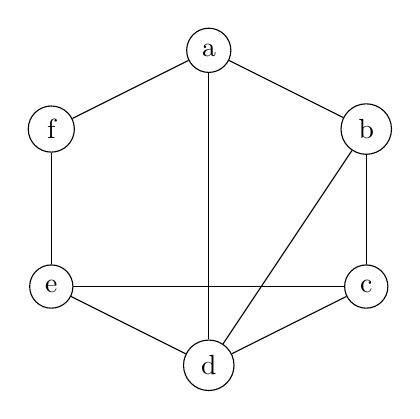
\begin{tikzpicture}[align=center, node distance=8cm,on grid]
   
   \node[shape=circle,draw=black] (1) at (0,0) {e};
   \node[shape=circle,draw=black] (2) at (0,2) {f};
   \node[shape=circle,draw=black] (3) at (4,0) {c};
   \node[shape=circle,draw=black] (4) at (4,2) {b};
   \node[shape=circle,draw=black] (5) at (2,3) {a};
   \node[shape=circle,draw=black] (6) at (2,-1) {d};
   

    \path[-] (1) edge node {} (2);
    \path[-] (2) edge node {} (5);
    \path[-] (3) edge node {} (4);
   	\path[-] (6) edge node {} (5);
   	\path[-] (4) edge node {} (5);
	\path[-] (1) edge node {} (3);
	\path[-] (1) edge node {} (6);
	\path[-] (3) edge node {} (6);
	\path[-] (4) edge node {} (6);
	
	\end{tikzpicture}
	
\subsection{Pseudocode}

\begin{algorithm}[H]
\textbf{begin}\\
 $q:=q_0$\\
 \For{$j:=1$ \KwTo $n$}{
 \While{$g[q,s_j]=$fail}{
  $q:=h[q]$\\
  \If{q is in F}{\KwRet{\enquote{yes}}

   }
 }
 \KwRet{\enquote{no}}
 }
 
 \caption{Fig. 9. The Aho-Corasik algorithm for matching multiple keywords}
\end{algorithm}




\end{document}
